
\newpage

\section*{Task 6}
In this section, a D Flip-Flop and a SR Latch
are implemented, based on logic gates.
\subsection*{SR Latch}
For the SR Latch, it is 
implemented using NOR gates of 74HC02 integrated
circuit. The resulting schematic is shown below.

\begin{figure}[H]
    \begin{centering}
    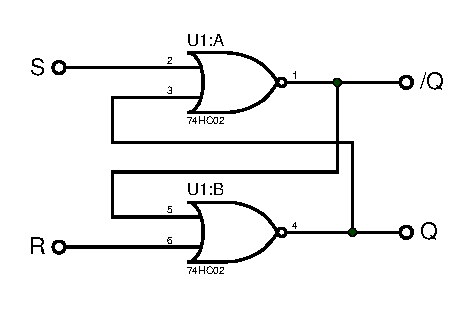
\includegraphics[width=0.5\textwidth]{data/latchSR}
    \par\end{centering}
    \caption{SR Latch circuit - Made in Proteus 7.8}
\end{figure}

The measured parameters are the same indicated
by the reference IC 74HC279\footnote{"TC74HC279AP", Toshiba, 1997-08-07} (Quad-SR-Latch): 
time propagation delays $(t_{pd})$ from S to Q, 
and from R to Q, for comparative purposes.

\begin{table}[H]
    \begin{center}
        \begin{tabular}{|c|c|c|c|c|}
            \hline 
            \multicolumn{2}{|c|}{PARAMETER} & FROM & TO & VALUE\tabularnewline
            \hline 
            \hline 
            \multirow{2}{*}{$t_{pd}$} & Circuit & S & Q & 13.2ns \tabularnewline
            \cline{2-5} 
             & 74HC279 & S & Q & 9ns\tabularnewline
            \hline 
            \multirow{2}{*}{$t_{pd}$} & Circuit & R & Q & 18ns \tabularnewline
            \cline{2-5} 
             & 74HC279 & R & Q & 11ns\tabularnewline
            \hline 
            \end{tabular}
    \caption{Measured values}
    \end{center}
\end{table}
As shown, the IC times are faster than the 
discrete latch builded. This diferences are 
related to the fact that the logic gates are 
not identical to each other, son they may have
diferent propagation delay times.\\
On the other side, with the Quad-NOT gate IC 74HC02 
only two latches can be built, in comparison with 
the four latches included in the 74HC279 IC.
\newpage
\subsection*{D Flip-Flop}
For the D flip-flop, it is implemented using 
the SR Latch designed before, adding the 
remaining parts as shown below.

\begin{figure}[H]
    \begin{centering}
    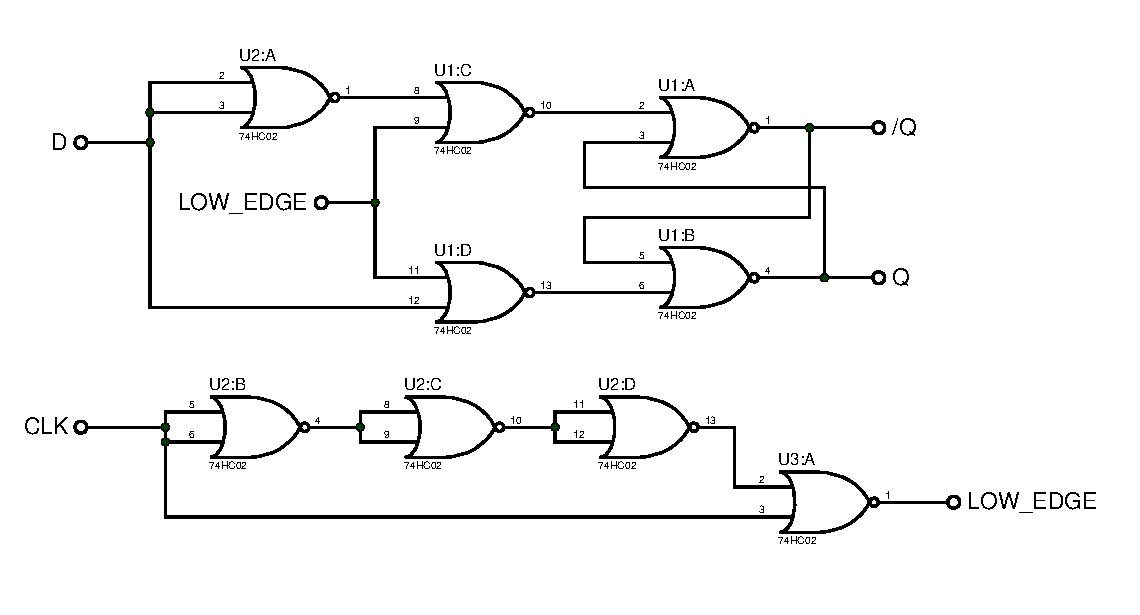
\includegraphics[width=0.8\textwidth]{data/dflipflop}
    \par\end{centering}
    \caption{D Flip-Flop circuit - Made in Proteus 7.8}
\end{figure}

The designed circuit will be compared with the 
74HC74\footnote{"74HC74 Dual D-type flip-flop with set and reset; positive edge-trigger", Nexperia, Rev.5 - 3 December 2015} D Flip-Flop.

\begin{table}[H]
    \begin{center}
        \begin{tabular}{|c|c|c|c|c|}
            \hline 
            \multicolumn{2}{|c|}{PARAMETER} & FROM & TO & VALUE\tabularnewline
            \hline 
            \hline 
            \multirow{2}{*}{$t_{pd}$} & Circuit & CLK & Q or /Q & 30ns\tabularnewline
            \cline{2-5} 
             & 74HC74 & CLK & Q or /Q & 14ns\tabularnewline
            \hline 
            \multirow{2}{*}{$t_t$} & Circuit &  & Q or /Q & 18ns \tabularnewline
            \cline{2-5} 
             & 74HC74 &  & Q or /Q & 7ns\tabularnewline
            \hline 
            \end{tabular}
    \caption{Measured values}
    \end{center}
\end{table}
As shown, the measured times from the built circuit 
are slower than the IC 74HC74 times. Also, it 
required two NOR-Gates IC (74HC02) to build the 
flip flop with all discrete logic gates, and 
each gate has its own time propagation delay that
needs to be considerated. On the other hand, the 
74HC74 has two flip flops in one IC; to build them 
with logic gates, 4 IC 74HC02 would be needed.
